\documentclass[handout]{beamer}


\usetheme{default}
\usepackage{subfigure}
\usepackage{Sweave}
\usepackage{graphicx}
%\usepackage{color}
\usepackage{multicol}
\usepackage{bm}


\author{Patrick Lam}
\title{Probability Theory}
\date{}
%\date{February 7, 2009}

\begin{document}

\newcommand{\red}{\textcolor{red}}
\newcommand{\blue}{\textcolor{blue}}
\newcommand{\purple}{\textcolor{purple}}

\frame{\titlepage}

\begin{frame}
\frametitle{Outline}
\tableofcontents
\end{frame}


\section{Probability}

\begin{frame}
Most Basic Definition of Probability:
\pause
\bigskip
\begin{eqnarray*}
\frac{\mathrm{number \; of \; successes}}{\mathrm{number \; of \; possible \; occurrences}}
\end{eqnarray*}
\end{frame}

\begin{frame}
\frametitle{Three Axioms of Probability}
\pause
Let $S$ be the sample space and $A$ be an event in $S$.
\pause
\medskip
\begin{enumerate}
\item For any event $A$, $P(A) \ge 0$.
\pause
\item $P(S) = 1$.
\pause
\item If $A_1, A_2, \dots, A_n$ are mutually disjoint, then
\begin{equation*}
P(A_1 \cup A_2 \cup \dots \cup A_n) = P(A_1) + P(A_2) + \dots + P(A_n)
\end{equation*}
\end{enumerate}
\pause
The three axioms imply:
\pause
\begin{itemize}
\item $P(\emptyset) = 0$
\pause
\item $P(A^c) = 1 - P(A)$
\pause
\item For any event $A$, $0 \le P(A) \le 1$.
\pause
\item If $A \subset B$, then $P(A) \le P(B)$.
\pause
\item For any two events $A$ and $B$, $P(A \cup B) = P(A) + P(B) - P(A
\cap B)$.
\end{itemize}
\end{frame}

\begin{frame}
\frametitle{Conditional Probability}
\pause
\begin{eqnarray*}
P(A|B) &=& \frac{P(A \cap B)}{P(B)} 
\end{eqnarray*}
\pause
Multiplicative Law of Probability:
\pause
\begin{eqnarray*}
P(A \cap B) = P(B|A) P(A) = P(A|B) P(B)
\end{eqnarray*}
\pause
Bayes' Rule:
\begin{eqnarray*}
\pause
P(A|B) &=& \frac{P(B|A) P(A)}{P(B)}
\end{eqnarray*}
\pause
Law of Total Probability:
\pause
\begin{eqnarray*}
P(B) = \sum_{i=1}^n P(B|A_i) P(A_i)
\end{eqnarray*}
\end{frame}

\begin{frame}
\frametitle{Independence}
$A$ and $B$ are independent if 
\begin{eqnarray*}
P(AB) = P(A) P(B)
\end{eqnarray*}
\pause
If $A$ and $B$ are independent, then
\begin{eqnarray*}
P(A|B) &=& \frac{P(AB)}{P(B)}\\
\pause
&=& \frac{P(A) P(B)}{P(B)} \\
\pause
&=& P(A)
\end{eqnarray*}
\pause
Conditional Independence:
\begin{eqnarray*}
P(AB | C) = P(A|C) P(B|C)
\end{eqnarray*}
\end{frame}

\section{Random Variables}


\begin{frame}
\frametitle{Outline}
\tableofcontents[currentsection]
\end{frame}

\begin{frame}
\frametitle{Random Variables}
\pause
A \textbf{random variable} is a function that takes a random experiment and
assigns a number to the outcome of the experiment. \\
\pause
\bigskip
Outcome values are assigned probabilities by a probability mass
function (for discrete RV) or probability density function (for
continuous RV).
\end{frame}

\begin{frame}
\frametitle{Probability Mass Function}
\pause
\begin{eqnarray*}
P(Y = y)
\end{eqnarray*}
\pause
\begin{figure}[!htp]
\begin{center}
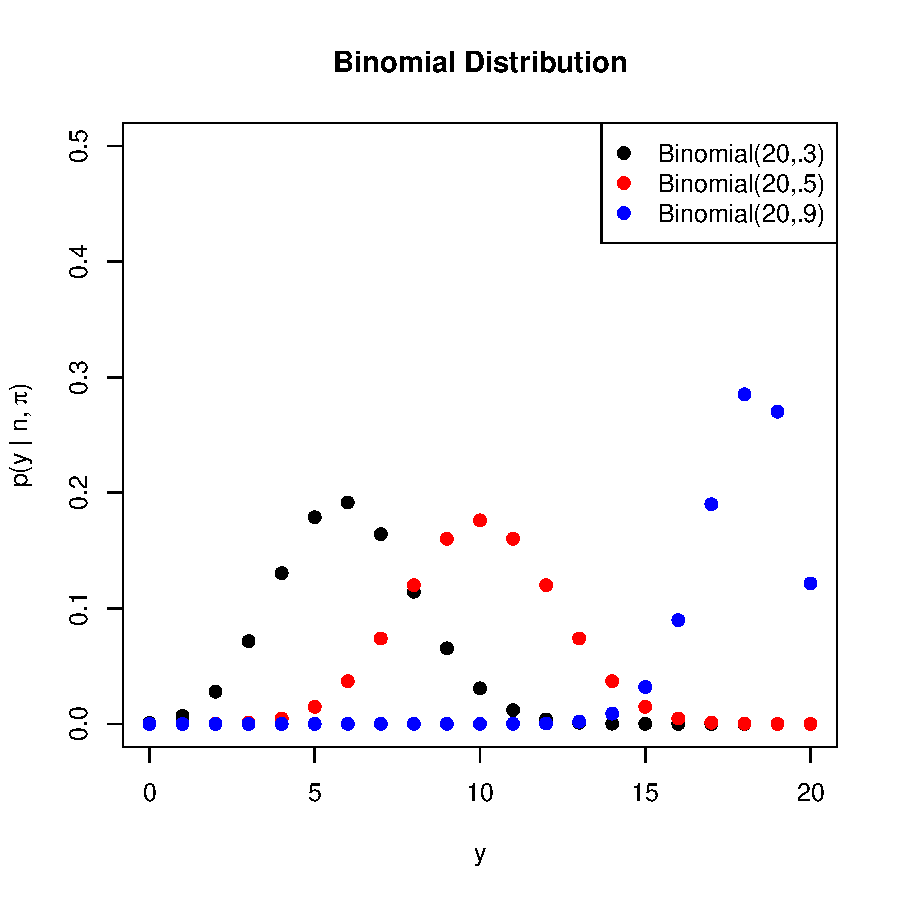
\includegraphics[width=2in, height=2in]{probability-binomial.pdf}
\end{center}
\end{figure}
\end{frame}

\begin{frame}
\frametitle{Probability Density Function}
\pause
\begin{eqnarray*}
P(Y \in A) = \int_A f(y) dy
\end{eqnarray*}
\pause
\begin{figure}[!htp]
\begin{center}
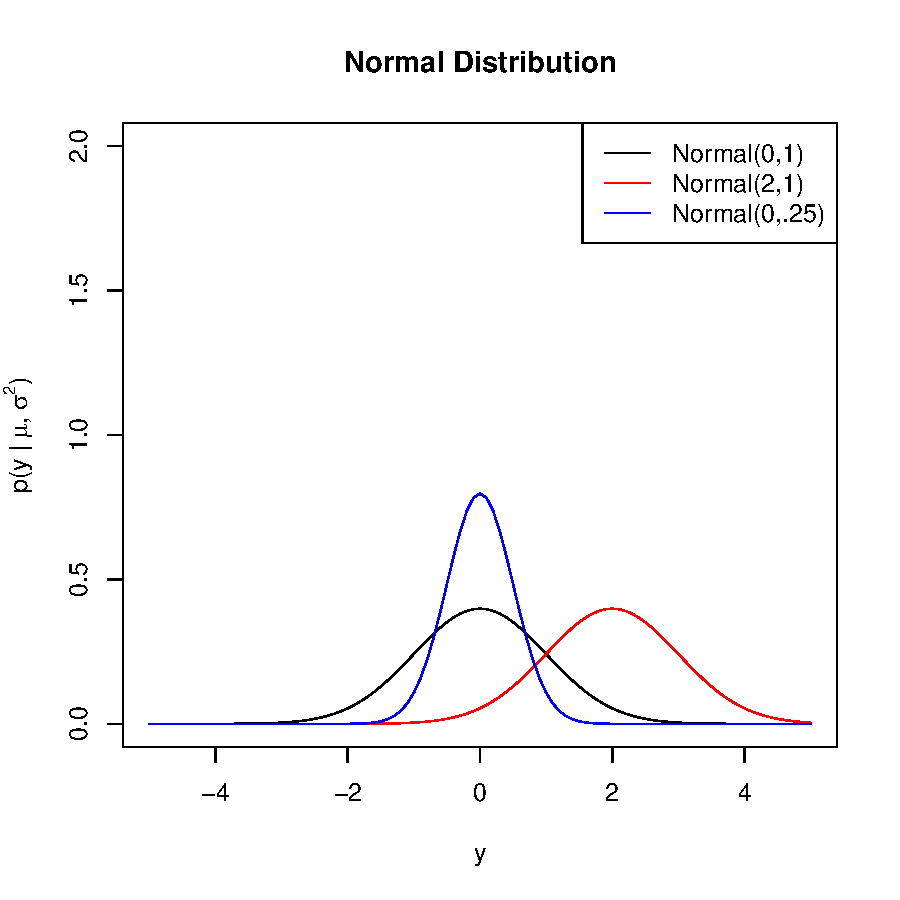
\includegraphics[width=2in, height=2in]{probability-normal.pdf}
\end{center}
\end{figure}
\end{frame}

\begin{frame}
Characteristics of all PDFs and PMFs:
\bigskip
\pause
\begin{itemize}
\item Area under the curve must integrate to 1
\pause
\item $P(Y = y) \ge 0$ for all $Y$
\pause
\item The support is all y's where $P(Y = y) > 0$.
\end{itemize}
\end{frame}

\begin{frame}
\frametitle{Marginal, Conditional, and Joint Densities}
\pause
\begin{eqnarray*}
f(x) &=& \int f(x,y) dy\\
\pause
f(x,y) &=& \int f(x,y,z) dz\\
\pause
f(x|y) &=& \frac{f(x,y)}{f(y)}\\
\pause
f(x|y,z) &=& \frac{f(x,y,z)}{f(y,z)}\\
\pause
f(x,y) &=& f(x | y) f(y)\\
\pause
&=& f(y | x) f(x) \\
\pause
f(x,y,z) &=& f(x | y,z) f(y|z) f(z)
\end{eqnarray*}
\end{frame}

\begin{frame}
\frametitle{Expectation}
%\pause
%The expected value of a random variable $X$ is simply the weighted
%average of all possible values of $X$.\\
%\bigskip
\pause
Discrete Case:
\pause
\begin{eqnarray*}
E(X) = \sum_i x_i P(X = x_i)
\end{eqnarray*}
where $P(X = x)$ is the probability mass function (PMF).\\
\pause
\bigskip
Continuous Case:
\pause
\begin{eqnarray*}
E(X) = \int^{\infty}_{-\infty} x f(x) dx
\end{eqnarray*}
where $f(x)$ is the probability density function (PDF).
\end{frame}

\begin{frame}
\frametitle{Expectation of a Function of a Random Variable}
%\pause
%Suppose we want to find $E[g(X)]$, where $g(X)$ is any function of
%$X$.  \pause  We can simply weight the values of $g(x)$ by the PDF or
%PMF of $X$:
\pause
\begin{eqnarray*}
E[g(X)] = \sum_i g(x_i) P(X = x_i)
\end{eqnarray*}
for discrete random variables \pause and 
\begin{eqnarray*}
E[g(X)] = \int_{-\infty}^{\infty} g(x) f(x) dx
\end{eqnarray*}
for continuous random variables.  \\
\bigskip
\pause
%This is sometimes known as the \textit{Law of the Unconscious
%Statistician} (LOTUS).
\end{frame}

\begin{frame}
\frametitle{Variance}
\pause
%The formula for the variance of a random variable is 
\begin{eqnarray*}
\mathrm{Var}(X) = E[(X - E(X))^2]
\end{eqnarray*}
\pause
%We can find the variance using LOTUS, \pause or we can simplify the
%formula first.
%\pause
\begin{eqnarray*}
\mathrm{Var}(X) &=& E[(X - E(X))^2]\\
\pause
&=& E[X^2 - 2 X E(X) + (E(X))^2]\\
\pause
&=& E(X^2) - 2 E(X) E[E(X)] + E([E(X)]^2)\\
\pause
&=& E(X^2) - 2 [E(X)]^2 + [E(X)]^2\\
\pause
&=& \mathbf{E(X^2) - [E(X)]^2}
\end{eqnarray*}
\pause
%We can then find the first part with LOTUS.
\end{frame}

\section{Simulation}

\begin{frame}
\frametitle{Outline}
\tableofcontents[currentsection]
\end{frame}

\begin{frame}
\frametitle{Monte Carlo Simulation}
\pause
All the simulations we will be doing in class is what we call
\textbf{Monte Carlo simulation}.
\pause
\begin{figure}[!htp]
\subfigure{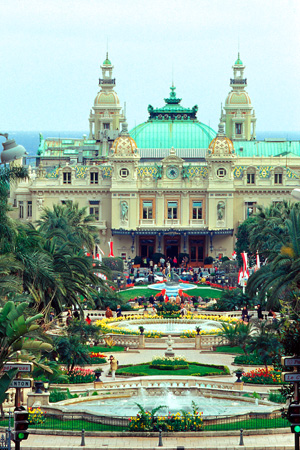
\includegraphics[width=1.5in, height=1.5in]{casino.jpg}}
\subfigure{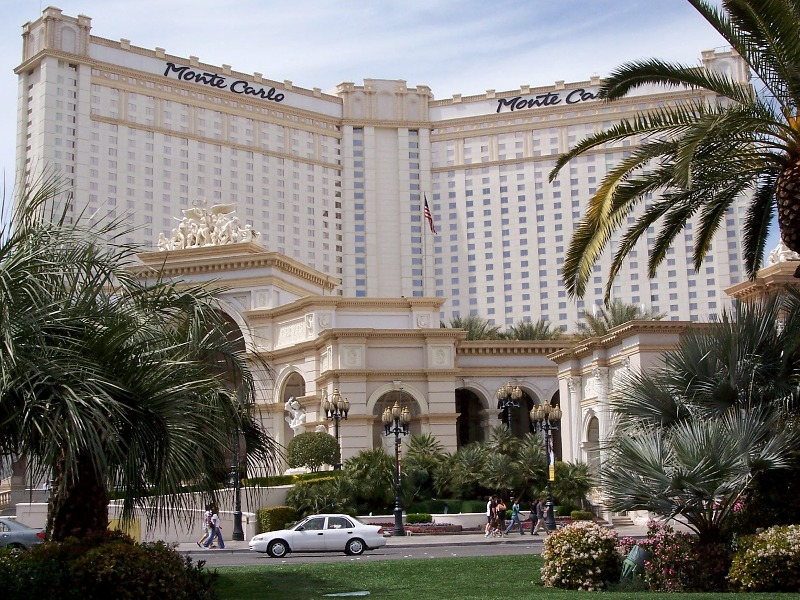
\includegraphics[width=1.5in, height=1.5in]{hotel.jpg}}
\end{figure}
\pause
Fancy way of saying we will simulate random draws to calculate
quantities of interest.
\end{frame}

\begin{frame}
\frametitle{Simulating from a Random Variable}
\pause
Suppose we have a random variable $X$ that follows a Beta($\alpha$,
$\beta$) distribution.
\pause
\begin{figure}[!htp]
\begin{center}
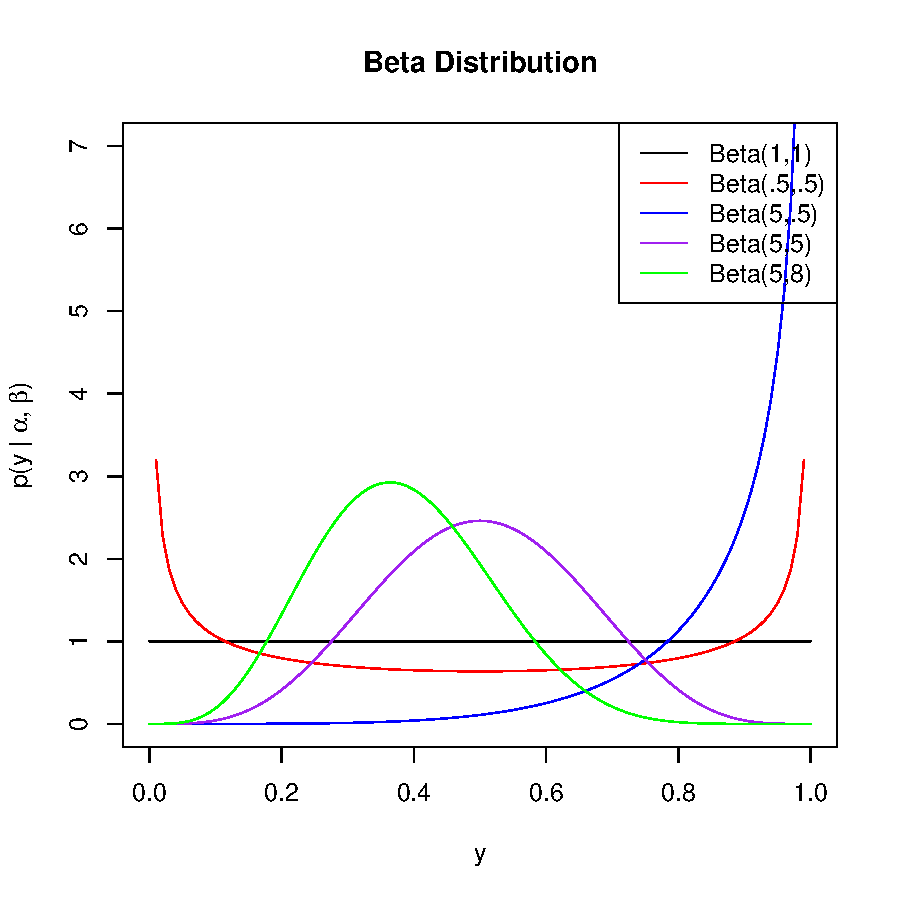
\includegraphics[width=2in, height=2in]{probability-beta.pdf}
\end{center}
\end{figure}
\pause
\begin{eqnarray*}
f(x| \alpha, \beta) = \frac{\Gamma (\alpha + \beta)}{\Gamma (\alpha)
\Gamma (\beta)} x^{(\alpha - 1)} (1 - x)^{(\beta-1)}\\
\end{eqnarray*}
\end{frame}

\begin{frame}[fragile]
Let $\alpha = 2$ and $\beta = 3$. Find $E(X)$.  
\pause
\begin{eqnarray*}
E(X) &=& \int^{1}_{0} x f(x) dx \\
\pause
&=&\int^{1}_{0} x \; \frac{\Gamma (\alpha + \beta)}{\Gamma (\alpha)
\Gamma (\beta)} x^{(\alpha - 1)} (1 - x)^{(\beta-1)} \\
\pause
&=&  \int^{1}_{0} x \; \frac{\Gamma (2 + 3)}{\Gamma (2)
\Gamma (3)} x^{(2 - 1)} (1 - x)^{(3-1)} dx \\
\end{eqnarray*}
\pause
We can ask R to help us integrate.
\tiny
\medskip
\pause
\begin{Schunk}
\begin{Sinput}
> ex.beta.func <- function(x, alpha, beta) {
+     x * gamma(alpha + beta)/(gamma(alpha) * gamma(beta)) * x^(alpha - 
+         1) * (1 - x)^(beta - 1)
+ }
> e.x <- integrate(Vectorize(ex.beta.func), lower = 0, upper = 1, 
+     alpha = 2, beta = 3)$value
> e.x
\end{Sinput}
\begin{Soutput}
[1] 0.4
\end{Soutput}
\end{Schunk}
\normalsize
\end{frame}

\begin{frame}[fragile]
Or we can use simulation, which is much easier.
\pause
\bigskip
\tiny
\begin{Schunk}
\begin{Sinput}
> x.draws <- rbeta(10000, shape1 = 2, shape2 = 3)
> sim.e.x <- mean(x.draws)
> sim.e.x
\end{Sinput}
\begin{Soutput}
[1] 0.3987049
\end{Soutput}
\end{Schunk}
\normalsize
\pause
\bigskip
We can find all kinds of quantities of interest (variance, quantiles,
etc.) by just doing it on the simulated draws rather than doing
complicated integrals. \\
\pause
\bigskip
Why does this work?
\end{frame}

\begin{frame}
\frametitle{Monte Carlo Integration}
\pause
What we just did was called \textbf{Monte Carlo Integration}, which
means exactly what it sounds like (doing integrals via Monte Carlo
simulation). \\
\pause
\bigskip
If we need to take an integral of the following form:
\begin{eqnarray*}
I = \int g(x) p(x) dx
\end{eqnarray*}
\pause
Monte Carlo Integration allows us to approximate it by simulating $M$
values from $f(x)$ and calculating:
\begin{eqnarray*}
\hat{I}_M = \frac{1}{M} \sum_{i=1}^M g(x^{(i)})
\end{eqnarray*}
\pause
By the Strong Law of Large Numbers, our estimate $\hat{I}_M$ is a simulation consistent estimator of $I$
as $M \rightarrow \infty$ \pause (our estimate gets better as we
increase the number of simulations).
\end{frame}

\begin{frame}[fragile]
Let $Y$ be another random variable where $Y = e^X$.  Find $E(Y)$.
\pause
\begin{eqnarray*}
E(Y) = \int^{1}_{0} e^x \; \frac{\Gamma (2 + 3)}{\Gamma (2)
\Gamma (3)} x^{(2 - 1)} (1 - x)^{(3-1)} dx \\
\end{eqnarray*}
\pause
Via simulation:
\medskip
\tiny
\pause
\begin{Schunk}
\begin{Sinput}
> e.y <- mean(exp(x.draws))
> e.y
\end{Sinput}
\begin{Soutput}
[1] 1.520348
\end{Soutput}
\end{Schunk}
\normalsize
\pause
\bigskip
Note that $E(g(X)) \neq g(E(X))$.  \pause In fact, $E(g(X)) \ge
g(E(X))$ by Jensen's Inequality.\\
\pause
\bigskip
Monte Carlo Integration tells us we need $E(g(X))$.
\end{frame}

\begin{frame}
Take home point: \\
\bigskip
\pause
If we can somehow generate random draws from the distribution of a
random variable, we can calculate complicated integrals (mean,
variance, functions of RV) easily by simulation. \\
\bigskip
\pause
This seems trivial but is one of the foundations of statistics,
especially Bayesian statistics.
\end{frame}

\begin{frame}
\frametitle{Simulating Probability Problems}
\pause
A related application of simulation is to help us solve probability problems.\\
\pause
\bigskip
General idea:
\pause
\begin{enumerate}
\item Suppose we have an experiment where we want to know the probability of
success.  Simulate from the population many times.
\pause
\item For each simulation, conduct the experiment and see whether there is success.
\pause
\item The proportion of simulations that achieve success is the
probability of success.
\end{enumerate}
\end{frame}

\begin{frame}[fragile]
\frametitle{An Example}
\pause
\small
Suppose we have two urns containing marbles.  The first urn contains 6
red marbles and 4 green marbles and the second urn contains 9 red
marbles and 1 green marble.  Take one marble from the first urn
(without looking at it) and put it in the second urn.  Then take one
marble from the second urn (again without looking at it) and put it in
the first urn.  What is the probability of now drawing a red marble
from the first urn?
\pause
\medskip
\tiny
\begin{Schunk}
\begin{Sinput}
> urn.func <- function(n.sims, urn1, urn2) {
+     final.draws <- c()
+     for (i in 1:n.sims) {
+         draw1 <- sample(urn1, 1)
+         draw2 <- sample(c(urn2, draw1), 1)
+         final.draws[i] <- sample(c(urn1, draw2), 1)
+     }
+     prob <- mean(final.draws)
+     return(prob)
+ }
> urn.func(n.sims = 10000, urn1 = c(rep(1, 6), rep(0, 4)), urn2 = c(rep(1, 
+     9), 0))
\end{Sinput}
\begin{Soutput}
[1] 0.6293
\end{Soutput}
\end{Schunk}
\pause
\color{red}
\begin{eqnarray*}
\left(\frac{6}{10} \right)\left(\frac{10}{11} \right)
\left(\frac{6}{10} \right) + \left(\frac{6}{10} \right)
\left(\frac{1}{11} \right) \left(\frac{5}{10} \right) +
\left(\frac{4}{10} \right) \left(\frac{9}{11} \right)
\left(\frac{7}{10} \right) + \left(\frac{4}{10} \right)
\left(\frac{2}{11} \right) \left(\frac{6}{10} \right) \approx 0.63
\end{eqnarray*}
\color{black}
\normalsize
\end{frame}

\begin{frame}[fragile]
\frametitle{Another Example}
\pause
\small
Suppose we have two urns containing marbles.  The first urn contains $10-g$
red marbles and $g$ green marbles and the second urn contains 9 red
marbles and 1 green marble.  Take one marble from the first urn
(without looking at it) and put it in the second urn.  Then take one
marble from the second urn (again without looking at it) and put it in
the first urn.  What is the minimum $g$ such that the probability of
now drawing a red marble is less than 0.5?
\pause
\medskip
\tiny
\begin{Schunk}
\begin{Sinput}
> urn.func2 <- function(n.sims, urn2, p) {
+     final.draws <- c()
+     g <- 0
+     urn1 <- c(rep(1, 10 - g), rep(0, g))
+     prob <- 1
+     while (prob >= p) {
+         for (i in 1:n.sims) {
+             draw1 <- sample(urn1, 1)
+             draw2 <- sample(c(urn2, draw1), 1)
+             final.draws[i] <- sample(c(urn1, draw2), 1)
+         }
+         prob <- mean(final.draws)
+         g <- g + 1
+         urn1 <- c(rep(1, 10 - g), rep(0, g))
+     }
+     g <- g - 1
+     return(g)
+ }
> urn.func2(1000, urn2 = c(rep(1, 9), 0), p = 0.5)
\end{Sinput}
\begin{Soutput}
[1] 6
\end{Soutput}
\end{Schunk}
\normalsize
\end{frame}

\section{Important Distributions}


\begin{frame}
\frametitle{Outline}
\tableofcontents[currentsection]
\end{frame}

\subsection{Discrete Distributions}


\begin{frame}
\frametitle{Outline}
\tableofcontents[currentsubsection]
\end{frame}

\begin{frame}
\frametitle{The Bernoulli Distribution}
\begin{multicols}{2}
\pause
$Y \sim$ Bernoulli$(\pi)$\\
\bigskip
\pause
$y = 0,1$\\
\bigskip
\pause
probability of success: $\pi \in [0,1]$\\
\bigskip
\pause
$p(y|\pi) = \pi^y (1 - \pi)^{(1-y)}$\\
\bigskip
\bigskip
\pause
$E(Y) = \pi$\\
\bigskip
\pause
Var$(Y) = \pi (1 - \pi)$
\pause


\begin{figure}[!htp]
\begin{center}
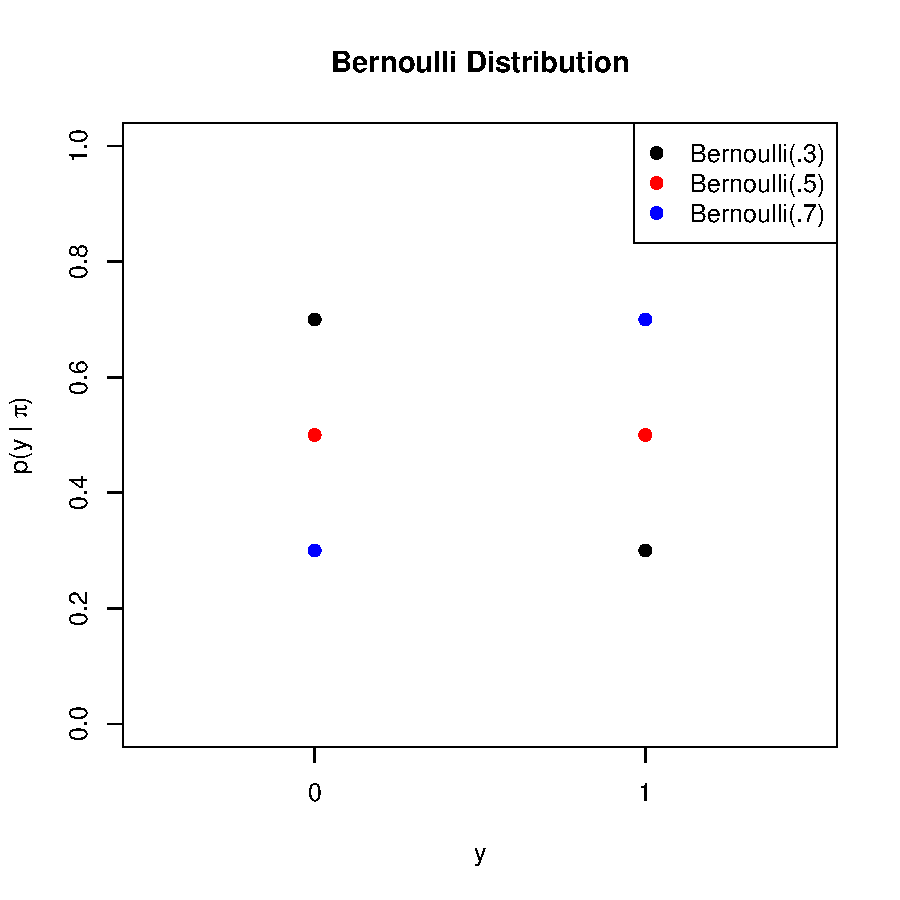
\includegraphics[width=2in, height=2in]{probability-bernoulli.pdf}
\end{center}
\end{figure}
\end{multicols}
\end{frame}



\begin{frame}
\frametitle{The Binomial Distribution}
\begin{multicols}{2}
\pause
$Y \sim$ Binomial$(n, \pi)$\\
\bigskip
\pause
$y = 0,1,\dots,n$\\
\bigskip
\pause
number of trials: $n \in \{1,2,\dots \}$\\
\pause
probability of success: $\pi \in [0,1]$\\
\bigskip
\pause
$p(y|\pi) = \binom{n}{y} \pi^y (1 - \pi)^{(n-y)}$\\
\bigskip
\bigskip
\pause
$E(Y) = n \pi$\\
\bigskip
\pause
Var$(Y) = n \pi (1 - \pi)$
\pause


\begin{figure}[!htp]
\begin{center}
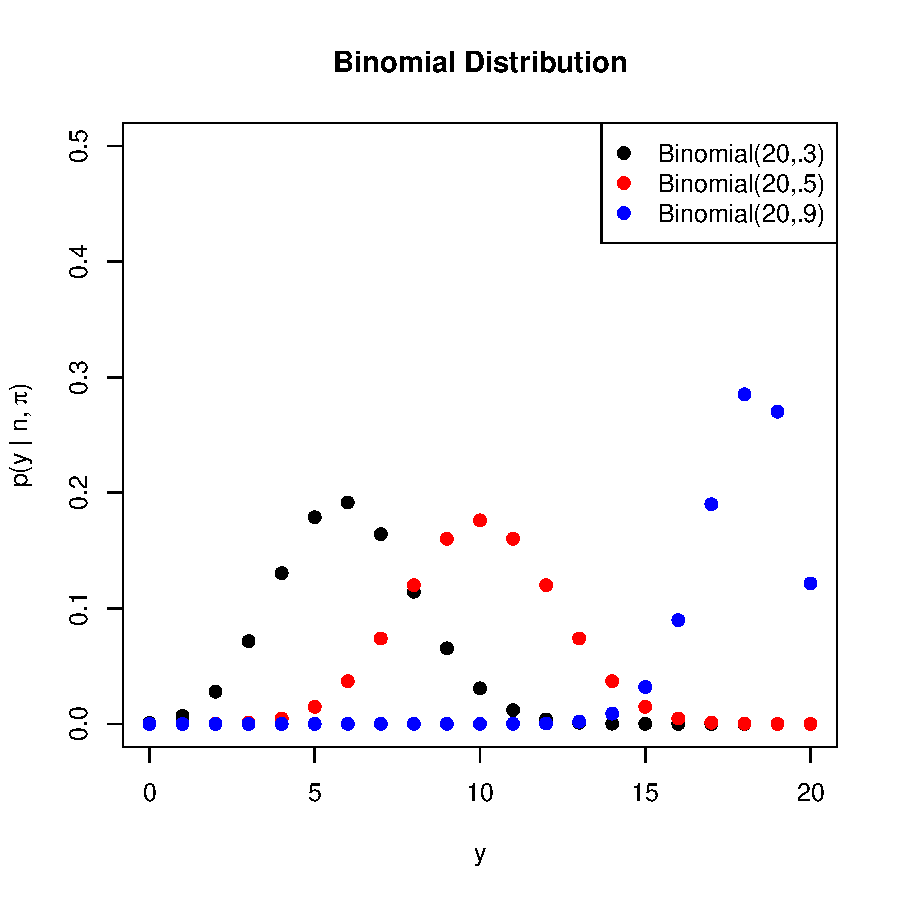
\includegraphics[width=2in, height=2in]{probability-binomial.pdf}
\end{center}
\end{figure}
\end{multicols}
\end{frame}


\begin{frame}
\frametitle{The Multinomial Distribution}
\pause
$Y \sim$ Multinomial$(n,\pi_1, \dots, \pi_k)$\\
\bigskip
\pause
$y_j = 0,1,\dots,n; \; \; \sum_{j=1}^k y_j = n$\\
\bigskip
\pause
number of trials: $n \in \{1,2,\dots \}$\\
\pause
probability of success for $j$: $\pi_j \in [0,1]; \; \; \sum_{j=1}^k
\pi_j = 1$\\
\bigskip
\pause
$p(\mathbf{y}|n,\bm{\pi}) = \frac{n!}{y_1! y_2! \dots
y_k!}\pi_1^{y_1}\pi_2^{y_2} \dots \pi_k ^ {y_k}$\\
\bigskip
\bigskip
\pause
$E(Y_j) = n\pi_j$\\
\bigskip
\pause
Var$(Y_j) = n \pi_j (1 - \pi_j)$\\
\bigskip
\pause
Cov$(Y_i, Y_j) = -n \pi_i \pi_j$


\end{frame}



\begin{frame}
\frametitle{The Poisson Distribution}
\begin{multicols}{2}
\pause
$Y \sim$ Poisson$(\lambda)$\\
\bigskip
\pause
$y = 0,1,\dots$\\
\bigskip
\pause
expected number of occurrences: $\lambda > 0$\\
\bigskip
\pause
$p(y|\lambda) = \frac{e^{-\lambda} \lambda^y}{y!}$\\
\bigskip
\bigskip
\pause
$E(Y) = \lambda$\\
\bigskip
\pause
Var$(Y) = \lambda$
\pause


\begin{figure}[!htp]
\begin{center}
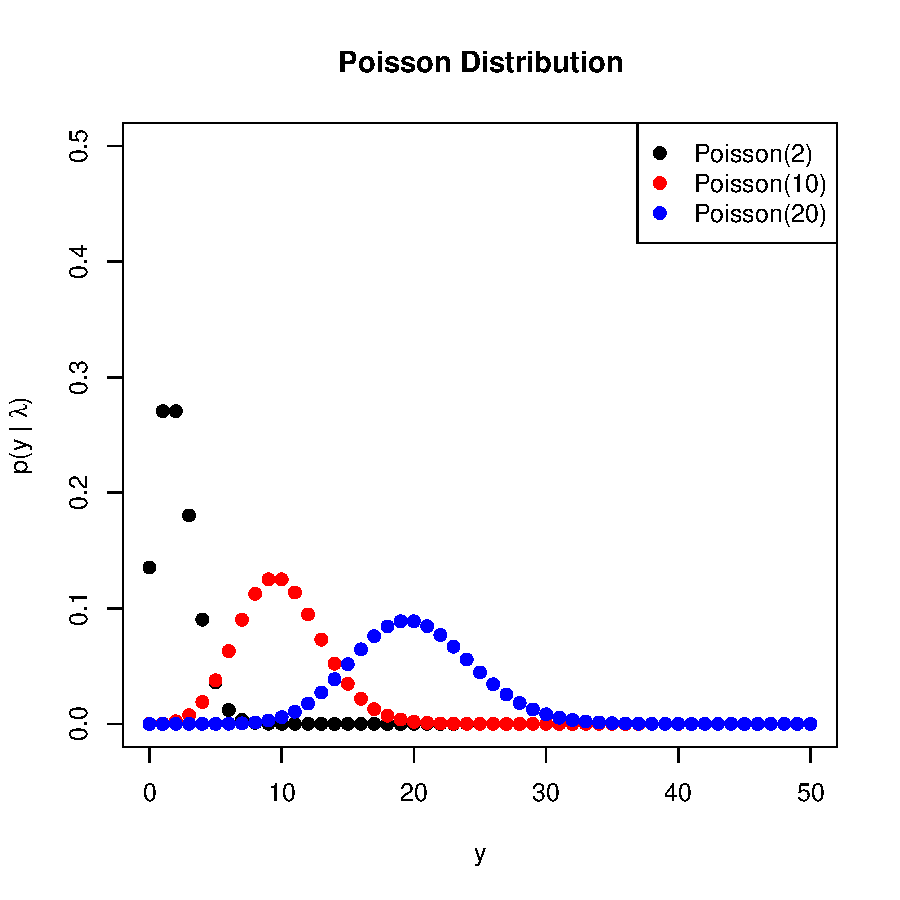
\includegraphics[width=2in, height=2in]{probability-poisson.pdf}
\end{center}
\end{figure}
\end{multicols}
\end{frame}

\begin{frame}
\frametitle{The Geometric Distribution}
\pause
How many Bernoulli trials until success?
\begin{multicols}{2}
\pause
$Y \sim$ Geometric$(\pi)$\\
\bigskip
\pause
$y = 1,2,3,\dots$\\
\bigskip
\pause
probability of success: $\pi \in [0,1]$\\
\bigskip
\pause
$p(y|\pi) = (1 - \pi)^{(y-1)} \pi$\\
\bigskip
\bigskip
\pause
$E(Y) = \frac{1}{\pi}$\\
\bigskip
\pause
Var$(Y) = \frac{1 - \pi}{\pi^2}$
\pause


\begin{figure}[!htp]
\begin{center}
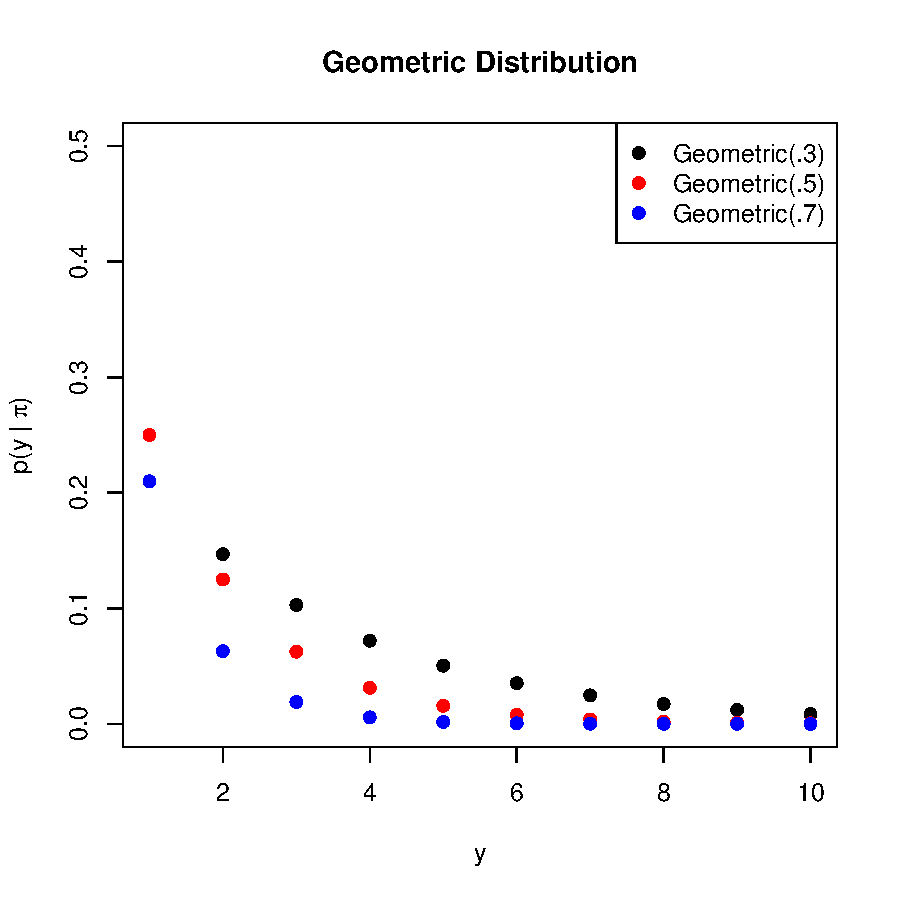
\includegraphics[width=2in, height=2in]{probability-geometric.pdf}
\end{center}
\end{figure}
\end{multicols}
\end{frame}

\subsection{Continuous Distributions}


\begin{frame}
\frametitle{Outline}
\tableofcontents[currentsubsection]
\end{frame}

\begin{frame}
\frametitle{The Univariate Normal Distribution}
\begin{multicols}{2}
\pause
$Y \sim$ Normal$(\mu, \sigma^2)$\\
\bigskip
\pause
$y \in \mathbb{R}$\\
\bigskip
\pause
mean: $\mu \in \mathbb{R}$\\
\pause
variance: $\sigma^2 > 0$\\
\bigskip
\pause
$p(y|\mu, \sigma^2) = \frac{\exp \left( {-\frac{(y - \mu)^2}{2\sigma^2} } \right)}{\sigma \sqrt{2 \pi}}$\\
\bigskip
\bigskip
\pause
$E(Y) = \mu$\\
\bigskip
\pause
Var$(Y) = \sigma^2$
\pause


\begin{figure}[!htp]
\begin{center}
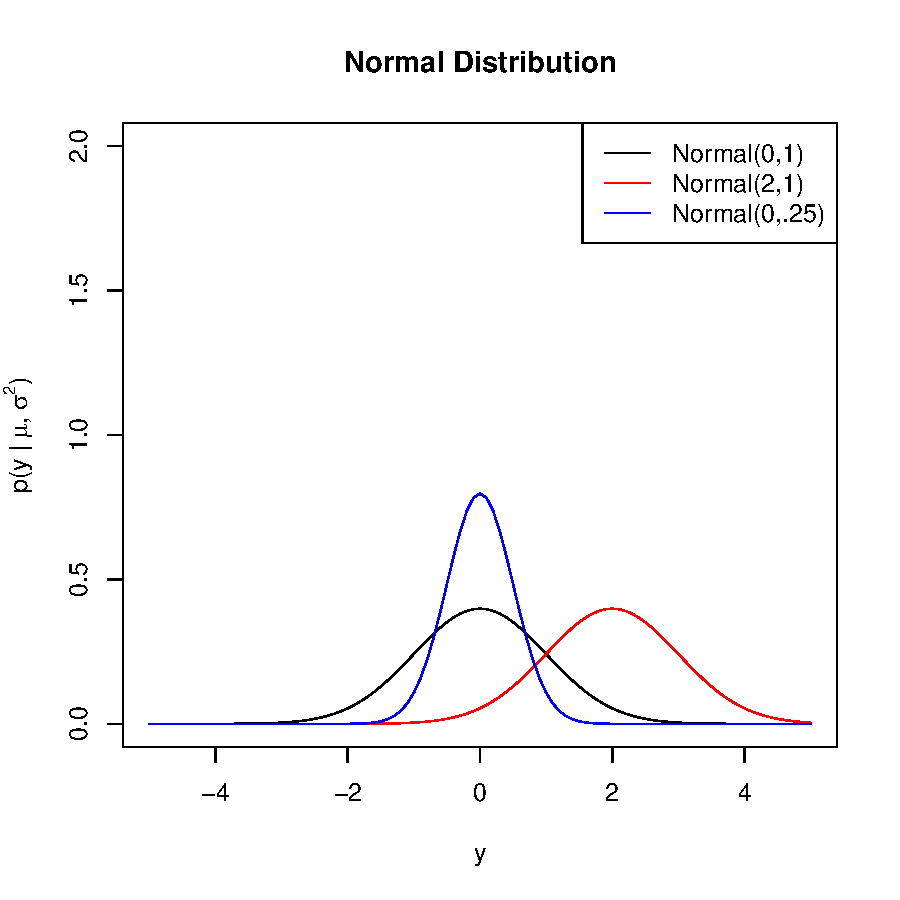
\includegraphics[width=2in, height=2in]{probability-normal.pdf}
\end{center}
\end{figure}
\end{multicols}
\end{frame}



\begin{frame}
\frametitle{The Multivariate Normal Distribution}
\pause
$Y \sim \mathcal{N}(\bm{\mu},\bm{\Sigma})$\\
\bigskip
\pause
$\mathbf{y} \in \mathbb{R}^k$\\
\bigskip
\pause
mean vector: $\bm{\mu} \in \mathbb{R}^k$\\
\pause
variance-covariance matrix: $\bm{\Sigma}$ positive definite $k \times
k$ matrix\\
\bigskip
\pause
$p(\mathbf{y}|\bm{\mu},\bm{\pi}) = (2\pi)^{-k/2} | \bm{\Sigma}
|^{-1/2} \exp{\left( -\frac{1}{2} (\bm{y} - \bm{\mu})'
\bm{\Sigma^{-1}} (\bm{y} - \bm{\mu}) \right)}$\\
\bigskip
\bigskip
\pause
$E(Y) = \bm{\mu}$\\
\bigskip
\pause
Var$(Y) = \bm{\Sigma}$\\
\end{frame}


\begin{frame}
\frametitle{The Uniform Distribution}
\pause
$Y \sim$ Uniform$(\alpha, \beta)$\\
\bigskip
\pause
$y \in [\alpha, \beta]$\\
\bigskip
\pause
Interval: $[\alpha, \beta]; \; \; \beta > \alpha$\\
\bigskip
\pause
$p(y| \alpha, \beta) = \frac{1}{\beta - \alpha}$\\
\bigskip
\bigskip
\pause
$E(Y) = \frac{\alpha + \beta}{2}$\\
\bigskip
\pause
Var$(Y) = \frac{(\beta - \alpha)^2}{12}$

\end{frame}



\begin{frame}
\frametitle{The Beta Distribution}
\begin{multicols}{2}
\pause
$Y \sim$ Beta$(\alpha, \beta)$\\
\bigskip
\pause
$y \in [0,1]$\\
\bigskip
\pause
shape parameters: $\alpha > 0; \; \; \beta > 0$\\
\bigskip
\pause
$p(y| \alpha, \beta) = \frac{\Gamma (\alpha + \beta)}{\Gamma (\alpha)
\Gamma (\beta)} y^{(\alpha - 1)} (1 - y)^{(\beta-1)}$\\
\bigskip
\bigskip
\pause
$E(Y) = \frac{\alpha}{\alpha + \beta}$\\
\bigskip
\pause
Var$(Y) = \frac{\alpha \beta}{(\alpha + \beta)^2 )\alpha + \beta + 1)}$


\begin{figure}[!htp]
\begin{center}
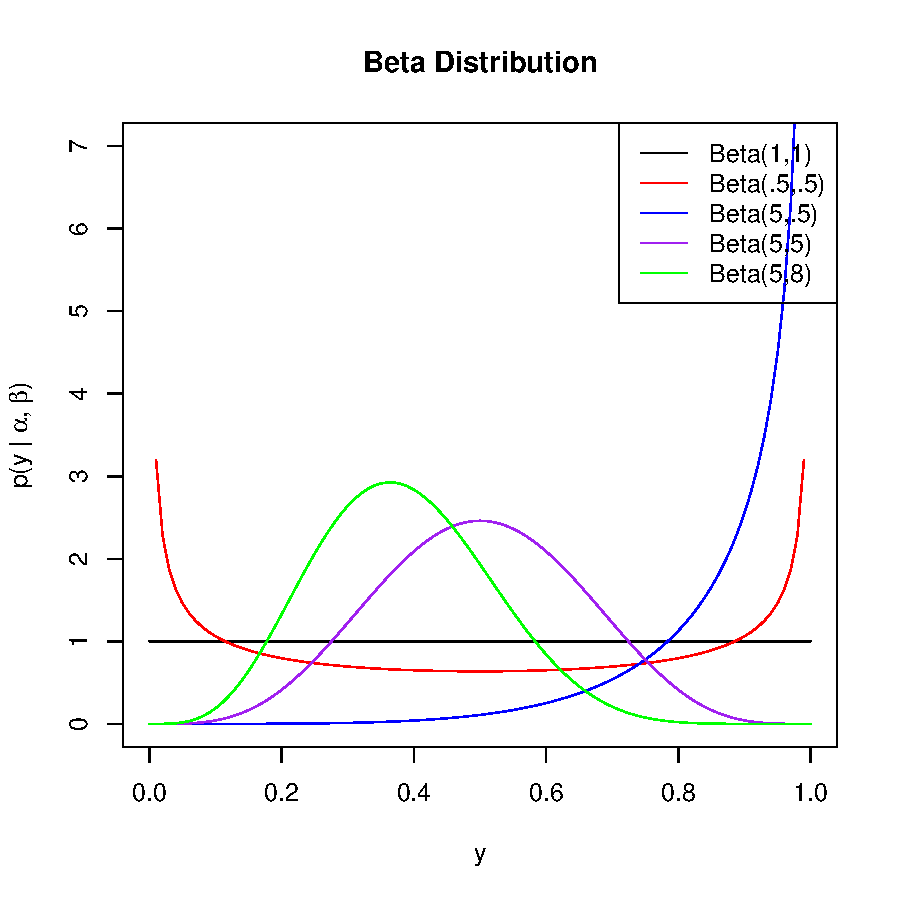
\includegraphics[width=2in, height=2in]{probability-beta.pdf}
\end{center}
\end{figure}
\end{multicols}

\end{frame}


\begin{frame}
\frametitle{The Gamma Distribution}
\pause
\begin{multicols}{2}
$Y \sim$ Gamma$(\alpha, \beta)$\\
\bigskip
\pause
$y > 0$\\
\bigskip
\pause
shape parameter: $\alpha > 0$\\
\pause
inverse scale parameter: $\beta > 0$ \\
\bigskip
\pause
$p(y| \alpha, \beta) = \frac{\beta^{\alpha}}{\Gamma (\alpha)}
y^{(\alpha - 1)} \exp{(-\beta y)}$\\
\bigskip
\bigskip
\pause
$E(Y) = \frac{\alpha}{\beta}$\\
\bigskip
\pause
Var$(Y) = \frac{\alpha}{\beta^2}$


\begin{figure}[!htp]
\begin{center}
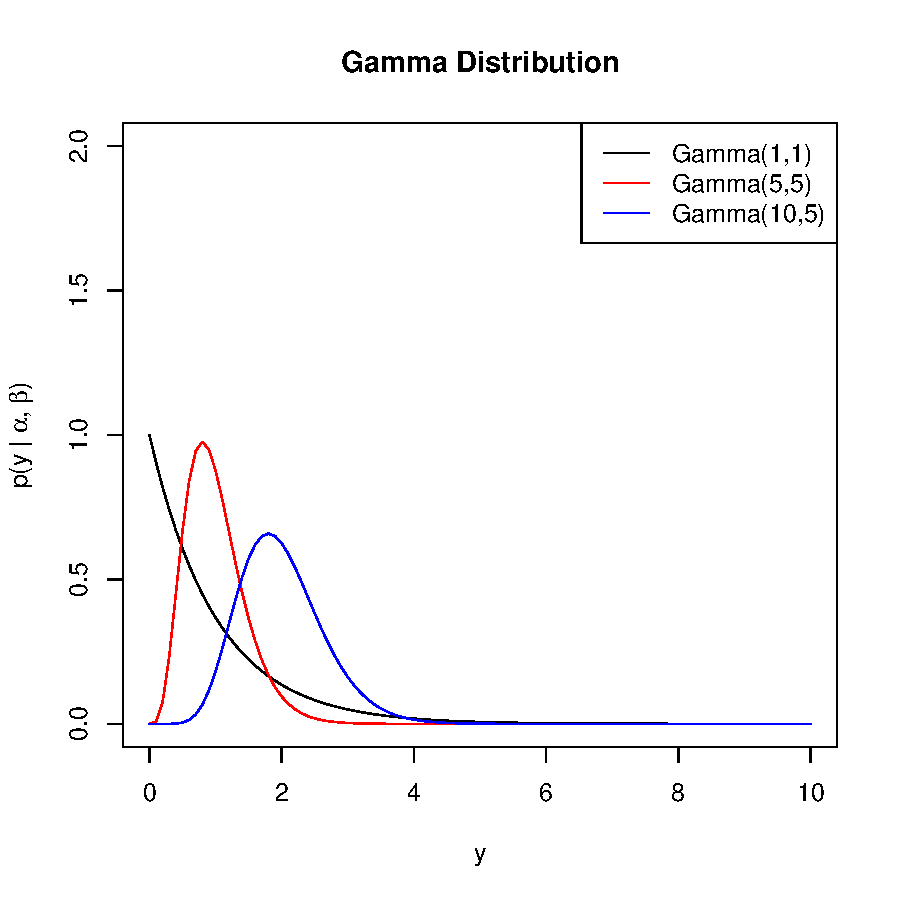
\includegraphics[width=2in, height=2in]{probability-gamma.pdf}
\end{center}
\end{figure}
\end{multicols}
\end{frame}


\begin{frame}
\frametitle{The Inverse Gamma Distribution}
\pause
Distribution of the Inverse of a Gamma Distribution: \pause If $X \sim$
Gamma($\alpha, \beta$), then $\frac{1}{X} \sim$ Invgamma($\alpha, \beta$).
\begin{multicols}{2}
\pause
$Y \sim$ Invgamma$(\alpha, \beta)$\\
\bigskip
\pause
$y > 0$\\
\bigskip
\pause
shape parameter: $\alpha > 0$\\
\pause
scale parameter: $\beta > 0$\\
\bigskip
\pause
$p(y|\alpha, \beta) = \frac{\beta^\alpha}{\Gamma(\alpha)}
y^{-(\alpha+1)} e^{-\frac{\beta}{y}}$\\
\bigskip
\bigskip
\pause
$E(Y) = \frac{\beta}{\alpha-1}$ for $\alpha > 1$\\
\bigskip
\pause
Var$(Y) = \frac{\beta^2}{(\alpha-1)^2 (\alpha-2)}$ for $\alpha > 2$
\pause


\begin{figure}[!htp]
\begin{center}
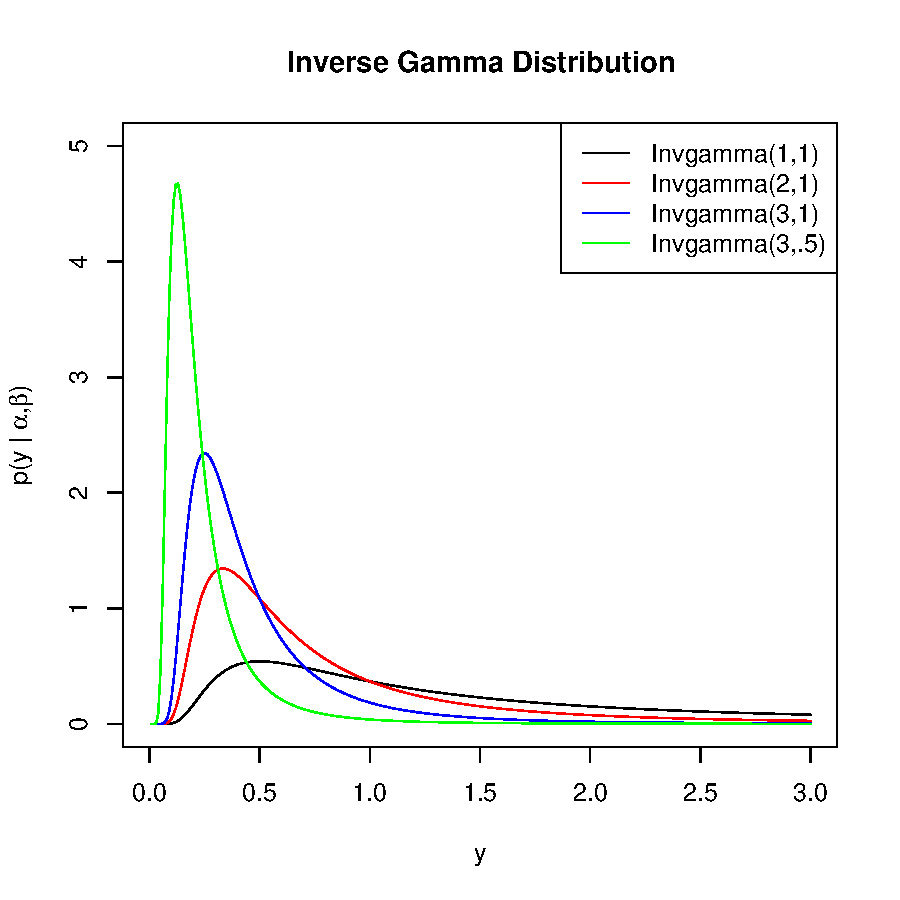
\includegraphics[width=2in, height=2in]{probability-invgamma.pdf}
\end{center}
\end{figure}
\end{multicols}
\end{frame}


\begin{frame}
\frametitle{The Dirichlet Distribution}
\pause
$Y \sim$ Dirichlet$(\alpha_1,\dots, \alpha_k)$\\
\bigskip
\pause
$y_j \in [0,1]; \; \; \sum_{j=1}^{k} y_j = 1$\\
\bigskip
\pause
$\alpha$ parameters: $\alpha_j > 0; \; \; \sum_{j=1}^k \alpha_j \equiv
\alpha_0$\\
\bigskip
\pause
$p(\mathbf{y}| \bm{\alpha}) = \frac{\Gamma (\alpha_1 + \dots +
\alpha_k)}{\Gamma (\alpha_1) \dots \Gamma (\alpha_k)} y_1^{\alpha_1 -
1} \dots y_k^{\alpha_k - 1}$\\
\bigskip
\bigskip
\pause
$E(Y_j) = \frac{\alpha_j}{\alpha_0}$\\
\bigskip
\pause
Var$(Y_j) = \frac{\alpha_j (\alpha_0 - \alpha_j)}{\alpha^2_0 (\alpha_0
+ 1)}$\\
\bigskip
\pause
Cov$(Y_i, Y_j) = -\frac{\alpha_i \alpha_j}{\alpha^2_0 (\alpha_0 + 1)}$
\end{frame}

\end{document}
